\documentclass[12pt,a4paper,final]{article}
\usepackage[hmargin=2cm,vmargin=2cm,bmargin=2cm]{geometry} % Margem Obrigatoria
\usepackage{pslatex} %times new roman obrigatorio
\usepackage{setspace}
\usepackage[utf8x]{inputenc}
\usepackage{ucs}
\usepackage{amsmath}
%\usepackage[•]{•}kage{amsfonts}
\usepackage{amssymb}
\usepackage{graphicx}
\usepackage{floatrow}
\usepackage{multirow}
\usepackage{indentfirst}
\usepackage{natbib}
\usepackage{listings}
\usepackage[brazil]{babel} % em portugues brasileiro
\floatsetup[table]{capposition=top} 
\author{Alexandre Brisighello - 101350 \\ Marcus Felipe Botacin - 103338}
\title{ChessPhi}
%\bibliographystyle{IEEEtran}
\renewcommand{\lstlistingname}{Listagem}


\begin{document}

\onehalfspace %Espaçamento 1.5 obrigatório

\maketitle
\newpage
\tableofcontents
\newpage

%\section{Resumo}

\section{Introdução}

O uso de computadores para tentar encontrar um bom movimento em um determinado jogo de xadrez já é feito há muitos anos e com vários algoritmos diferentes . Um deles, que também pode ser aplicado para outros jogos, chama-se \textit{Alpha-Beta-Pruning}, que visa melhorar a performance do \textit{Minimax}, sem permitir a perda do melhor resultado.

O foco deste trabalho é a implementação serial e paralela de um programa que, fazendo uso do algoritmo citado, visa obter um bom próximo movimento. Ambas implementações são feitas em C, sendo a paralela para a plataforma Xeon Phi. Para fazer a integração destes dois trechos, será implementada também uma simples interface do jogo em Python, que dará a opção ao jogador se este quer ou não uma dica para a próxima jogada, além de permitir a configuração da computação que será feita (número máximo de profundidade ou tempo de processamento, por exemplo). 

\section{Implementação}

\subsection{Interface}

A interface em Python é baseada na biblioteca QtPython, funcionando através de um sistema de \textit{grid}. Os primeiros 8x8 elementos são \textit{labels} exibindo as peças no tabuleiro, e os demais são botões de controle. 

As peças no tabuleiro são imagens carregadas a partir da matriz-tabuleiro. Esta matriz é mantida pelo programa em Python e é independente dos módulos serial e paralelo. Esta matriz pode ser atualizada livremente ou através da execução/chamada dos módulos seriais e/ou paralelos.

A chamada dos módulos em C é feita através da chamada de um processo através da biblioteca subprocess. A matriz mantida em memória é passada como entrada via linha de comando e é atualizada com o resultado do tabuleiro \textit{parsed} de \textit{stdout}.

\subsection{Serial}

O algoritmo serial consiste basicamente de um backtracking dos movimentos possiveis, realizados sequencialmente, até que toda a computação acabe ou que se tenha atingido algum um limite de tempo/profundidade pré-estabelecido. Nota-se que já existem diversas classificações para determinar o valor de cada peça do jogo, sendo utilizada uma já existente. A pontuação será calculada da seguinte forma:

\begin{equation}
Score = \sum_{Peças de A} val(peças) - \sum_{Peças de B} val(peças)
\end{equation}

\begin{figure}[H]
\centering
\label{fig1}
\caption{\textit{Alpha Beta Pruning}}
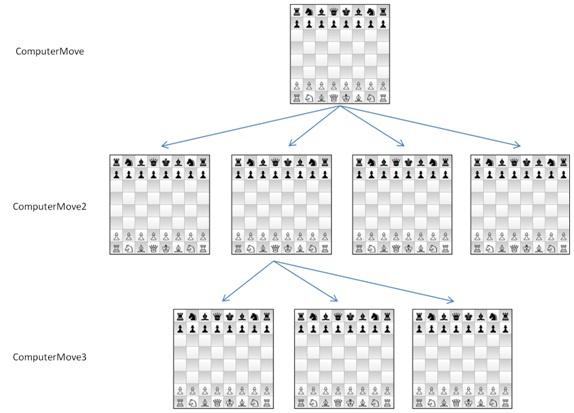
\includegraphics[scale=1]{../presentation/huoChess_2.jpg}
\end{figure}

O funcionamento do alfa-beta-pruning (como mostrado na figura~\ref{fig1})  permite a eliminação de algumas sub-árvores, melhorando o desempenho em relação ao Min-Max. A implementação proposta foi projetada de modo a eliminar recursões e alocação de memória, diminuindo a quantidade de memória utilizada e melhorando o desempenho. Estas características facilitaram a implementação paralela, sendo que a versão serial é usada pelas threads da versão paralela.

\subsection{Paralela}

Devido a estrutura das arquiteturas usadas e do algoritmo, foi feito uso de Pthreads, onde se implementou algo similar a ideia de \textit{Bag Of Tasks}, visando sempre obter uma árvore com a maior altura possível, já que, quanto maior a árvore, mais jogadas foram verificadas. A comunicação com Xeon Phi é feita através de SSH.

Decidiu - se por abrir os 2 primeiros níveis da árvore em \textit{threads}, correspondendo a 1 jogada de cada um dos jogadores. Em média, se tem 20 novos movimentos a cada rodada, o que gera, em média, 400 \textit{threads}.

Cada uma destas \textit{threads} executa o algoritmo serial para uma profundidade diminuidade de 2, se aproveitando da implementação serial em cada uma destas chamadas.

Na implementação paralela, as \textit{threads} são criadas de antemão e funcionam num sistema semelhante a uma máquina de estados. No primeiro estado, a \textit{thread} principal gera os movimentos do próximo nível enquanto as \textit{worker threads} aguardam por trabalho, num sistema semelhante a produtor-consumidor. A partir de então, a \textit{thread} principal aguardar para recolher o resultado de todas as \textit{ẁorker threads (reduction)}.

No segundo estado, as \textit{worker threads} abrem o segundo nível, e também aguardam para realizar o \textit{reduction} destes. Os estados 3 e 4 são os \textit{reduction} em si, os quais são feitos por \textit{Min} e \textit{Max}, respectivamente, dado o algoritmo \textit{Minimax}. Se todas as \textit{threads} atingem o nível 4 e não há mais trabalho, o \textit{join} é realizado. Todas as barreiras foram implementadas com \textit{mutex+semaphore}.

\section{Testes}

Para efetuar a comparação entre as duas implementações, foi feito um pequeno benchmark consistente de 5 jogos pré estabelecidos onde o programa busca pelo próximo movimento que garante a vitória do jogador (checkmate). O programa vai aumentando a profundidade de execução até que essa jogada seja encontrada, medindo o tempo de execução do início da busca até o final, onde a jogada é encontrada.

\subsection{Benchmarks}

Selecionamos 4 casos (posicionamento de peças no tabuleiro) equivalentes a jogadas interessantes, isto é, que tenham um \textit{check} após algumas rodadas. Os algoritmos da tabela~\ref{tab1} foram executados com incremento de \textit{depth} até que o \textit{check} fosse encontrado.

\begin{table}[h]
	\label{tab1}
	\centering
	\caption{Resultados (Tempo em segundos)}
	\label{my-label}
	\begin{tabular}{|l|l|l|l|l|}
		\hline
		Algorítmo            & Benchmark 1 & Benchmark 2 & Benchmark 3 & Benchmark 4 \\ \hline
		Min-Max Serial       & a           & a           & a           & a           \\ \hline
		Alpha Beta Serial    & a           & a           & a           & a           \\ \hline
		Alpha Beta O2 Serial & a           & a           & a           & a           \\ \hline
		Alpha Beta O3 Serial & a           & a           & a           & a           \\ \hline
		Paralelo 4 Threads   & a           & a           & a           & a           \\ \hline
		Paralelo 8 Threads   & a           & a           & a           & a           \\ \hline
		Xeon Phi             & a           & a           & a           & a           \\ \hline
	\end{tabular}
\end{table}

AlphaBetaxMinMAx~\cite{chess2}
alpha beta hard~\cite{chess1}

%\bibliographystyle{IEEEtran}  
\bibliographystyle{alpha}
\bibliography{projeto.bib}
\end{document}
